\documentclass{article}[12pt]

% useful packages
\usepackage{titlesec}
\usepackage{fullpage}
\usepackage{amsmath,amssymb,amsthm,amsfonts}
\usepackage{graphicx}
\usepackage{enumerate}
\usepackage{algorithm,algorithmic}
\usepackage{xcolor}
\usepackage{bbm}
\usepackage{url}
\usepackage{hyperref}

% theorem type environments
\newtheorem{thm}{Theorem}
\newtheorem{prop}{Proposition}
\newtheorem{lemma}{Lemma}
\newtheorem{cor}{Corollary}
\newtheorem{defn}{Definition}
\newtheorem{assump}{Assumption}
\newtheorem{example}{Example}
\newtheorem{conjecture}{Conjecture}

% frequently used symbols
\newcommand{\bE}{\mathbb{E}}
\newcommand{\bP}{\mathbb{P}}
\newcommand{\bQ}{\mathbb{Q}}
\newcommand{\bR}{\mathbb{R}}
\newcommand{\bS}{\mathbb{S}}
\newcommand{\bN}{\mathbb{N}}
\newcommand{\bZ}{\mathbb{Z}}
\newcommand{\sC}{{\mathcal C}} 
\newcommand{\sD}{{\mathcal D}} 
\newcommand{\sE}{{\mathcal E}} 
\newcommand{\sF}{{\mathcal F}} 
\newcommand{\sL}{{\mathcal L}} 
\newcommand{\sH}{{\mathcal H}} 
\newcommand{\sN}{{\mathcal N}} 
\newcommand{\sO}{{\mathcal O}} 
\newcommand{\sP}{{\mathcal P}} 
\newcommand{\sR}{{\mathcal R}} 
\newcommand{\sS}{{\mathcal S}}
\newcommand{\sU}{{\mathcal U}} 
\newcommand{\sX}{{\mathcal X}} 
\newcommand{\sY}{{\mathcal Y}} 
\newcommand{\sZ}{{\mathcal Z}}

% operators
\newcommand{\sign}{\mathop{\mathrm{sign}}}
\newcommand{\supp}{\mathop{\mathrm{supp}}} % support
\newcommand{\argmin}{\operatornamewithlimits{arg\ min}}
\newcommand{\argmax}{\operatornamewithlimits{arg\ max}}
\newcommand{\dist}{\operatorname{dist}}
\newcommand{\tr}{\text{tr}}
\newcommand{\vecop}{\text{vec}}
\newcommand{\st}{\operatorname{s.t.}}
\newcommand{\cut}{\setminus}
\newcommand{\ind}[1]{\mathbbm{1}\left\{#1\right\}} 
\newcommand{\given}{\ | \ }

% grouping operators
\newcommand{\brac}[1]{\left[#1\right]}
\newcommand{\set}[1]{\left\{#1\right\}}
\newcommand{\abs}[1]{\left\lvert #1 \right\rvert}
\newcommand{\paren}[1]{\left(#1\right)}
\newcommand{\norm}[1]{\left\|#1\right\|}
\newcommand{\ip}[2]{\left\langle #1,#2 \right\rangle}

% code commands
\newcommand{\matlab}{\textsc{Matlab }}
\newcommand{\python}{\textsc{Python }}
\newcommand{\todo}[1]{\textcolor{red}{#1}}

% header command
\newcommand{\project}[3]{
    \pagestyle{myheadings}
    \thispagestyle{plain}
    \newpage
    \setcounter{page}{1}
    \setlength{\headsep}{10mm}
    \noindent
    \begin{center}
    \framebox{
        \vbox{\vspace{2mm}
            \hbox to 6.28in { {\bf EE 519: Deep Learning Theory \& Fundamentals
            \hfill Spring \the\year} }
        \vspace{4mm}
        \hbox to 6.28in { {\Large \hfill Mini Project #1 \hfill} }
        \vspace{2mm}
        \hbox to 6.28in { \Large \hfill Due: #2, 11:59PM PT \hfill }
        \vspace{2mm}
        \hbox to 6.28in { {\it Student Name: #3} \hfill {\it Instructor Name: John Lipor}}
        \vspace{2mm}}
   }
   \end{center}
   \markboth{Mini Project #1}{Mini Project #1}
   \vspace*{4mm}
}

\begin{document}

% PUT YOUR NAME BELOW WHERE I HAVE \X
\project{1}{April 28, \the\year}{Andy Franck}
% PUT YOUR NAME ABOVE WHERE I HAVE \X

\section*{Problem Description}

The objective of this project is to first train a Convolutional Neural Network capable of accurately categorizing geothermal heat flow residuals into one of four disctinct classes. After categorizing, the model will be studied using guided backpropogation to determine whether the trained model is utilizing certain structural settings to make its predictions (i.e. changes in elevation and topography). \\
The model will be trained on a detrended elevation map, partitioned into 222, 200x200 pixel images. For each patch, the label is the maximum residual value among all wells in the patch.\\
Although it would be convenient for the model to accurately predict a high percentage of labels, it is unlikely to happen with the limited data size. This report aims to develop a model that can accurately predict the labels with a reasonable degree of accuracy, and then analyze the model's behavior to determine whether it is utilizing the desired structural features to make its predictions.\\
Even without perfect model accuracy, the model can still be useful in determining what topographic features are most useful for predicting geothermal heat flow. This will lead to a better understanding of the relationship between topography and geothermal heat flow, and will help to inform future research.\\


\section*{Exploratory Data Analysis}

Because of the nature of the data, it was not necessary to perform much data analysis. 


\section*{Challenges}

The largest challenge of the project was the limited data size. With only 222 images, it was very difficult to make a model train properly and accurately predict labels. This was especially true when using a CNN, which requires a large amount of data.\\


\section*{Approach}

The initial step in devlopment involved developing a baseline Network in Network model as described in the d2l textbook. This initial model was used to determine whether the data was being processed correctly, and to determine whether the model was capable of learning. This model was trained for 100 epochs, and overfit the data considerably: \\

\begin{center}
    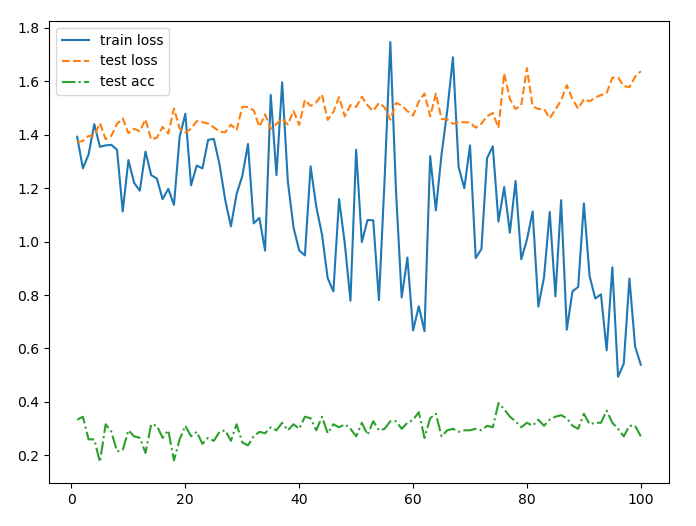
\includegraphics[width=0.5\textwidth]{images/basic_model.png}
\end{center}

The model also did not appear to be learning very well at all. The loss function was not decreasing, and the accuracy was not increasing. This was likely due to the small data size.\\

To artifically increase the data size, image augmentation was utilized via the torchvision.transforms library. This library allows for the creation of a transform object that can be applied to a dataset. The transform object contained both random flips and rotations at random degrees. The transform was applied after loading each batch at the start of the training loop, so that each batch was augmented differently. After applying the transform, the model appeared to train slightly better, but still did not appear to be learning very well:\\

\begin{center}
    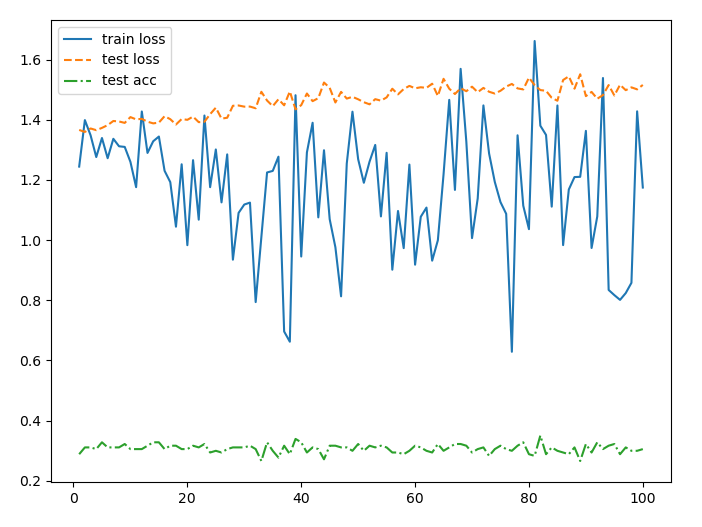
\includegraphics[width=0.5\textwidth]{images/basic_model_augmented.png}
\end{center}

The model still appeared to be overfitting, so dropout was added after each Network in Network block. This helped to reduce the overfitting, however the model did not improve in accuracy much:\\

\begin{center}
    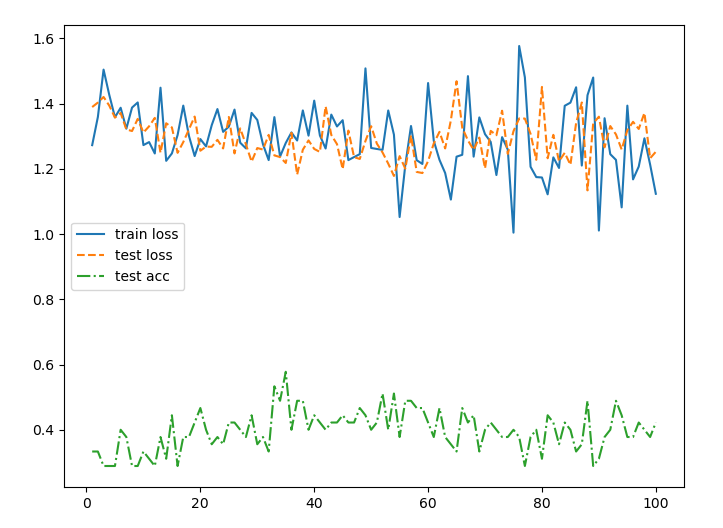
\includegraphics[width=0.5\textwidth]{images/model_augmented_dropout.png}
\end{center}


\section*{Evaluation and Summary}


\section*{What I Learned}


\bibliographystyle{IEEEtran}
\bibliography{bibliography}

\end{document}